% interactcadsample.tex
% v1.03 - April 2017

\documentclass[]{interact}

\usepackage{epstopdf}% To incorporate .eps illustrations using PDFLaTeX, etc.
\usepackage{subfigure}% Support for small, `sub' figures and tables
%\usepackage[nolists,tablesfirst]{endfloat}% To `separate' figures and tables from text if required

\usepackage{natbib}% Citation support using natbib.sty
\bibpunct[, ]{(}{)}{;}{a}{}{,}% Citation support using natbib.sty
\renewcommand\bibfont{\fontsize{10}{12}\selectfont}% Bibliography support using natbib.sty

\theoremstyle{plain}% Theorem-like structures provided by amsthm.sty
\newtheorem{theorem}{Theorem}[section]
\newtheorem{lemma}[theorem]{Lemma}
\newtheorem{corollary}[theorem]{Corollary}
\newtheorem{proposition}[theorem]{Proposition}

\theoremstyle{definition}
\newtheorem{definition}[theorem]{Definition}
\newtheorem{example}[theorem]{Example}

\theoremstyle{remark}
\newtheorem{remark}{Remark}
\newtheorem{notation}{Notation}

% see https://stackoverflow.com/a/47122900
\usepackage{color}
\usepackage{fancyvrb}
\newcommand{\VerbBar}{|}
\newcommand{\VERB}{\Verb[commandchars=\\\{\}]}
\DefineVerbatimEnvironment{Highlighting}{Verbatim}{commandchars=\\\{\}}
% Add ',fontsize=\small' for more characters per line
\usepackage{framed}
\definecolor{shadecolor}{RGB}{248,248,248}
\newenvironment{Shaded}{\begin{snugshade}}{\end{snugshade}}
\newcommand{\AlertTok}[1]{\textcolor[rgb]{0.94,0.16,0.16}{#1}}
\newcommand{\AnnotationTok}[1]{\textcolor[rgb]{0.56,0.35,0.01}{\textbf{\textit{#1}}}}
\newcommand{\AttributeTok}[1]{\textcolor[rgb]{0.77,0.63,0.00}{#1}}
\newcommand{\BaseNTok}[1]{\textcolor[rgb]{0.00,0.00,0.81}{#1}}
\newcommand{\BuiltInTok}[1]{#1}
\newcommand{\CharTok}[1]{\textcolor[rgb]{0.31,0.60,0.02}{#1}}
\newcommand{\CommentTok}[1]{\textcolor[rgb]{0.56,0.35,0.01}{\textit{#1}}}
\newcommand{\CommentVarTok}[1]{\textcolor[rgb]{0.56,0.35,0.01}{\textbf{\textit{#1}}}}
\newcommand{\ConstantTok}[1]{\textcolor[rgb]{0.00,0.00,0.00}{#1}}
\newcommand{\ControlFlowTok}[1]{\textcolor[rgb]{0.13,0.29,0.53}{\textbf{#1}}}
\newcommand{\DataTypeTok}[1]{\textcolor[rgb]{0.13,0.29,0.53}{#1}}
\newcommand{\DecValTok}[1]{\textcolor[rgb]{0.00,0.00,0.81}{#1}}
\newcommand{\DocumentationTok}[1]{\textcolor[rgb]{0.56,0.35,0.01}{\textbf{\textit{#1}}}}
\newcommand{\ErrorTok}[1]{\textcolor[rgb]{0.64,0.00,0.00}{\textbf{#1}}}
\newcommand{\ExtensionTok}[1]{#1}
\newcommand{\FloatTok}[1]{\textcolor[rgb]{0.00,0.00,0.81}{#1}}
\newcommand{\FunctionTok}[1]{\textcolor[rgb]{0.00,0.00,0.00}{#1}}
\newcommand{\ImportTok}[1]{#1}
\newcommand{\InformationTok}[1]{\textcolor[rgb]{0.56,0.35,0.01}{\textbf{\textit{#1}}}}
\newcommand{\KeywordTok}[1]{\textcolor[rgb]{0.13,0.29,0.53}{\textbf{#1}}}
\newcommand{\NormalTok}[1]{#1}
\newcommand{\OperatorTok}[1]{\textcolor[rgb]{0.81,0.36,0.00}{\textbf{#1}}}
\newcommand{\OtherTok}[1]{\textcolor[rgb]{0.56,0.35,0.01}{#1}}
\newcommand{\PreprocessorTok}[1]{\textcolor[rgb]{0.56,0.35,0.01}{\textit{#1}}}
\newcommand{\RegionMarkerTok}[1]{#1}
\newcommand{\SpecialCharTok}[1]{\textcolor[rgb]{0.00,0.00,0.00}{#1}}
\newcommand{\SpecialStringTok}[1]{\textcolor[rgb]{0.31,0.60,0.02}{#1}}
\newcommand{\StringTok}[1]{\textcolor[rgb]{0.31,0.60,0.02}{#1}}
\newcommand{\VariableTok}[1]{\textcolor[rgb]{0.00,0.00,0.00}{#1}}
\newcommand{\VerbatimStringTok}[1]{\textcolor[rgb]{0.31,0.60,0.02}{#1}}
\newcommand{\WarningTok}[1]{\textcolor[rgb]{0.56,0.35,0.01}{\textbf{\textit{#1}}}}

% Pandoc citation processing

\usepackage{hyperref}
\usepackage[utf8]{inputenc}
\def\tightlist{}


\begin{document}

\articletype{CLASS PROJECT}

\title{Taylor \& Francis Rmarkdown template for authors (\LaTeX-based
\textsf{Interact} layout + Chicago author-date reference style)}


\author{\name{Edwin Kagereki$^{a}$}
\affil{$^{a}$Taylor \& Francis, 4 Park Square, Milton Park, Abingdon,
UK}
}

\thanks{CONTACT Edwin
Kagereki. Email: \href{mailto:kagereki@dal.ca}{\nolinkurl{kagereki@dal.ca}}}

\maketitle

\begin{abstract}
This template is for authors who are preparing a manuscript for a Taylor
\& Francis journal using the \LaTeX~document preparation system and the
`interact\} class file, which is available via selected journals' home
pages on the Taylor \& Francis website.
\end{abstract}

\begin{keywords}
Sections; lists; figures; tables; mathematics; fonts; references;
appendices
\end{keywords}

\hypertarget{introduction}{%
\section{Introduction}\label{introduction}}

In order to assist authors in the process of preparing a manuscript for
a journal, the Taylor \& Francis `\textsf{Interact}' layout style has
been implemented as a \LaTeXe~class file based on the \texttt{article}
document class. A \textsc{Bib}\TeX~bibliography style file and a sample
bibliography are also provided in order to assist with the formatting of
your references.

Commands that differ from or are provided in addition to standard
\LaTeXe~are described in this document, which is \emph{not} a substitute
for a \LaTeXe~tutorial.

The \texttt{interactcadsample.tex} file can be used as a template for a
manuscript by cutting, pasting, inserting and deleting text as
appropriate, using the preamble and the \LaTeX~environments provided
(e.g.~\texttt{\textbackslash{}begin\{abstract\}},
\texttt{\textbackslash{}begin\{keywords\}}).

\hypertarget{the-class-file}{%
\subsection{\texorpdfstring{The \textsf{Interact} class
file}{The  class file}}\label{the-class-file}}

The \texttt{interact} class file preserves the standard
\LaTeXe~interface such that any document that can be produced using
\texttt{article.cls} can also be produced with minimal alteration using
the \texttt{interact} class file as described in this document.

If your article is accepted for publication it will be typeset as the
journal requires in Minion Pro and/or Myriad Pro. Since most authors
will not have these fonts installed, the page make-up is liable to alter
slightly with the change of font. Also, the \texttt{interact} class file
produces only single-column format, which is preferred for peer review
and will be converted to two-column format by the typesetter if
necessary during preparation of the proofs. Please therefore do not try
to match the typeset format exactly, but use the standard \LaTeX~fonts
instead and ignore details such as slightly long lines of text or
figures/tables not appearing in exact synchronization with their
citations in the text: these details will be dealt with by the
typesetter. Similarly, it is unnecessary to spend time addressing
warnings in the log file -- if your .tex file compiles to produce a PDF
document that correctly shows how you wish your paper to appear, such
warnings will not prevent your source files being imported into the
typesetter's program.

\hypertarget{submission-of-manuscripts-prepared-using}{%
\subsection{\texorpdfstring{Submission of manuscripts prepared using
\emph{\LaTeX}}{Submission of manuscripts prepared using }}\label{submission-of-manuscripts-prepared-using}}

Manuscripts for possible publication should be submitted to the Editors
for review as directed in the journal's Instructions for Authors, and in
accordance with any technical instructions provided in the journal's
ScholarOne Manuscripts or Editorial Manager site. Your \LaTeX~source
file(s), the class file and any graphics files will be required in
addition to the final PDF version when final, revised versions of
accepted manuscripts are submitted.

Please ensure that any author-defined macros used in your article are
gathered together in the preamble of your .tex file, i.e.~before the
\texttt{\textbackslash{}begin\{document\}} command. Note that if serious
problems are encountered in the coding of a document (missing
author-defined macros, for example), the typesetter may resort to
rekeying it.

\hypertarget{using-the-interact-class-file}{%
\section{\texorpdfstring{Using the \texttt{interact} class
file}{Using the interact class file}}\label{using-the-interact-class-file}}

For convenience, simply copy the \texttt{interact.cls} file into the
same directory as your manuscript files (you do not need to install it
in your \TeX~distribution). In order to use the \texttt{interact}
document class, replace the command
\texttt{\textbackslash{}documentclass\{article\}} at the beginning of
your document with the command
\texttt{\textbackslash{}documentclass\{interact\}}.

The following document-class options should \emph{not} be used with the
\texttt{interact} class file:

\begin{itemize}
\tightlist
\item
  \texttt{10pt}, \texttt{11pt}, \texttt{12pt} -- unavailable;
\item
  \texttt{oneside}, \texttt{twoside} -- not necessary, \texttt{oneside}
  is the default;
\item
  \texttt{leqno}, \texttt{titlepage} -- should not be used;
\item
  \texttt{twocolumn} -- should not be used (see
  Subsection\textasciitilde{}\ref{class});
\item
  \texttt{onecolumn} -- not necessary as it is the default style.
\end{itemize}

To prepare a manuscript for a journal that is printed in A4 (two column)
format, use the \texttt{largeformat} document-class option provided by
\texttt{interact.cls}; otherwise the class file produces pages sized for
B5 (single column) format by default. The \texttt{geometry} package
should not be used to make any further adjustments to the page
dimensions.

\hypertarget{additional-features-of-the-interact-class-file}{%
\section{\texorpdfstring{Additional features of the \texttt{interact}
class
file}{Additional features of the interact class file}}\label{additional-features-of-the-interact-class-file}}

\hypertarget{title-authors-names-and-affiliations-abstracts-and-article-types}{%
\subsection{Title, authors' names and affiliations, abstracts and
article
types}\label{title-authors-names-and-affiliations-abstracts-and-article-types}}

\hypertarget{abbreviations}{%
\subsection{Abbreviations}\label{abbreviations}}

A list of abbreviations may be included if required, enclosed within an
\texttt{abbreviations} environment,
i.e.~\texttt{\textbackslash{}begin\{abbreviations\}}\ldots\texttt{\textbackslash{}end\{abbreviations\}},
immediately following the \texttt{abstract} environment.

\hypertarget{keywords}{%
\subsection{Keywords}\label{keywords}}

A list of keywords may be included if required, enclosed within a
\texttt{keywords} environment,
i.e.~\texttt{\textbackslash{}begin\{keywords\}}\ldots\texttt{\textbackslash{}end\{keywords\}}.
Additional keywords in other languages (preceded by a translation of the
word \texttt{keywords}) may also be included within the
\texttt{keywords} environment if required.

\hypertarget{subject-classification-codes}{%
\subsection{Subject classification
codes}\label{subject-classification-codes}}

AMS, JEL or PACS classification codes may be included if required. The
\texttt{interact} class file provides an \texttt{amscode} environment,
i.e.~\texttt{\textbackslash{}begin\{amscode\}}\ldots\texttt{\textbackslash{}end\{amscode\}},
a \texttt{jelcode} environment,
i.e.~\texttt{\textbackslash{}begin\{jelcode\}}\ldots\texttt{\textbackslash{}end\{jelcode\}},
and a \texttt{pacscode} environment,
i.e.~\texttt{\textbackslash{}begin\{pacscode\}}\ldots\texttt{\textbackslash{}end\{pacscode\}}
to assist with this.

\hypertarget{additional-footnotes-to-the-title-or-authors-names}{%
\subsection{Additional footnotes to the title or authors'
names}\label{additional-footnotes-to-the-title-or-authors-names}}

Note that any \texttt{footnote}s to the main text will automatically be
assigned the superscript symbols 1, 2, 3, etc. by the class
file.\footnote{If preferred, the \texttt{endnotes} package may be used
  to set the notes at the end of your text, before the bibliography. The
  symbols will be changed to match the style of the journal if necessary
  by the typesetter.}

\hypertarget{embedding-r-code}{%
\section{Embedding R code}\label{embedding-r-code}}

\hypertarget{code-chunks}{%
\subsection{Code chunks}\label{code-chunks}}

\begin{Shaded}
\begin{Highlighting}[]
\FunctionTok{summary}\NormalTok{(cars)}
\end{Highlighting}
\end{Shaded}

\begin{verbatim}
##      speed           dist       
##  Min.   : 4.0   Min.   :  2.00  
##  1st Qu.:12.0   1st Qu.: 26.00  
##  Median :15.0   Median : 36.00  
##  Mean   :15.4   Mean   : 42.98  
##  3rd Qu.:19.0   3rd Qu.: 56.00  
##  Max.   :25.0   Max.   :120.00
\end{verbatim}

\hypertarget{including-plots}{%
\subsection{Including Plots}\label{including-plots}}

You can also embed plots, for example:

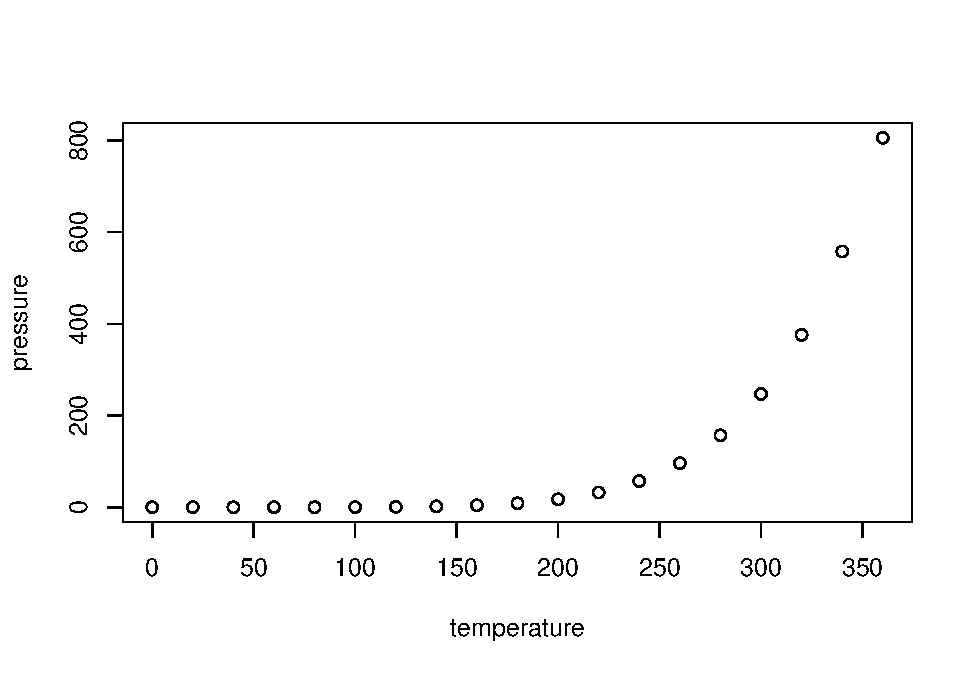
\includegraphics[width=0.8\linewidth]{Untitled_files/figure-latex/pressure-1}

Note that the \texttt{echo\ =\ FALSE} parameter was added to the code
chunk to prevent printing of the R code that generated the plot.

\hypertarget{some-guidelines-for-using-the-standard-features-of}{%
\section{\texorpdfstring{Some guidelines for using the standard features
of
\LaTeX}{Some guidelines for using the standard features of }}\label{some-guidelines-for-using-the-standard-features-of}}

\hypertarget{sections}{%
\subsection{Sections}\label{sections}}

The \textsf{Interact} layout style allows for five levels of section
heading, all of which are provided in the \texttt{interact} class file
using the standard \LaTeX~commands \texttt{\textbackslash{}section},
\texttt{\textbackslash{}subsection},
\texttt{\textbackslash{}subsubsection},
\texttt{\textbackslash{}paragraph} and
\texttt{\textbackslash{}subparagraph}. Numbering will be automatically
generated for all these headings by default.

\hypertarget{lists}{%
\subsection{Lists}\label{lists}}

Numbered lists are produced using the \texttt{enumerate} environment,
which will number each list item with arabic numerals by default. For
example,

\begin{enumerate}
\def\labelenumi{\arabic{enumi}.}
\tightlist
\item
  first item
\item
  second item
\item
  third item
\end{enumerate}

Alternative numbering styles can be achieved by inserting an optional
argument in square brackets to each \texttt{item},
e.g.~\texttt{\textbackslash{}item{[}(i){]}\ first\ item}, to create a
list numbered with roman numerals at level one.

Bulleted lists are produced using the \texttt{itemize} environment. For
example,

\begin{itemize}
\tightlist
\item
  First bulleted item
\item
  Second bulleted item
\item
  Third bulleted item
\end{itemize}

\hypertarget{figures}{%
\subsection{Figures}\label{figures}}

\begin{Shaded}
\begin{Highlighting}[]
\FunctionTok{plot}\NormalTok{(pressure)}
\end{Highlighting}
\end{Shaded}

The \texttt{interact} class file will deal with positioning your figures
in the same way as standard \LaTeX. It should not normally be necessary
to use the optional \texttt{{[}htb{]}} location specifiers of the
\texttt{figure} environment in your manuscript; you may, however, find
the \texttt{{[}p{]}} placement option or the \texttt{endfloat} package
useful if a journal insists on the need to separate figures from the
text.

Figure captions appear below the figures themselves, therefore the
\texttt{\textbackslash{}caption} command should appear after the body of
the figure. For example, Figure\textasciitilde{}\ref{sample-figure} with
caption and sub-captions is produced using the following commands:

\begin{verbatim}
\begin{figure}
\centering
\subfigure[An example of an individual figure sub-caption.]{%
\resizebox*{5cm}{!}{\includegraphics{path/to/fig}}}\hspace{5pt}
\subfigure[A slightly shorter sub-caption.]{%
\resizebox*{5cm}{!}{\includegraphics{path/to/fig}}}
\caption{Example of a two-part figure with individual sub-captions
 showing that captions are flush left and justified if greater
 than one line of text.} \label{sample-figure}
\end{figure}
\end{verbatim}

\begin{figure}
\centering
\subfigure[An example of an individual figure sub-caption.]{%
\resizebox*{5cm}{!}{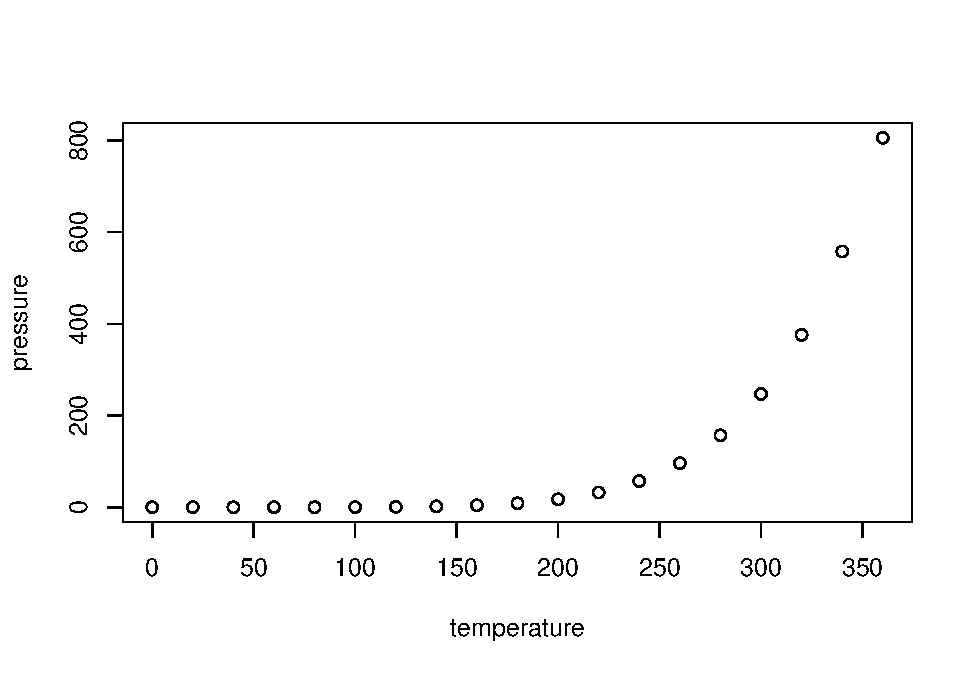
\includegraphics{Untitled_files/figure-latex/pressure-plot-1.pdf}}}\hspace{5pt}
\subfigure[A slightly shorter sub-caption.]{%
\resizebox*{5cm}{!}{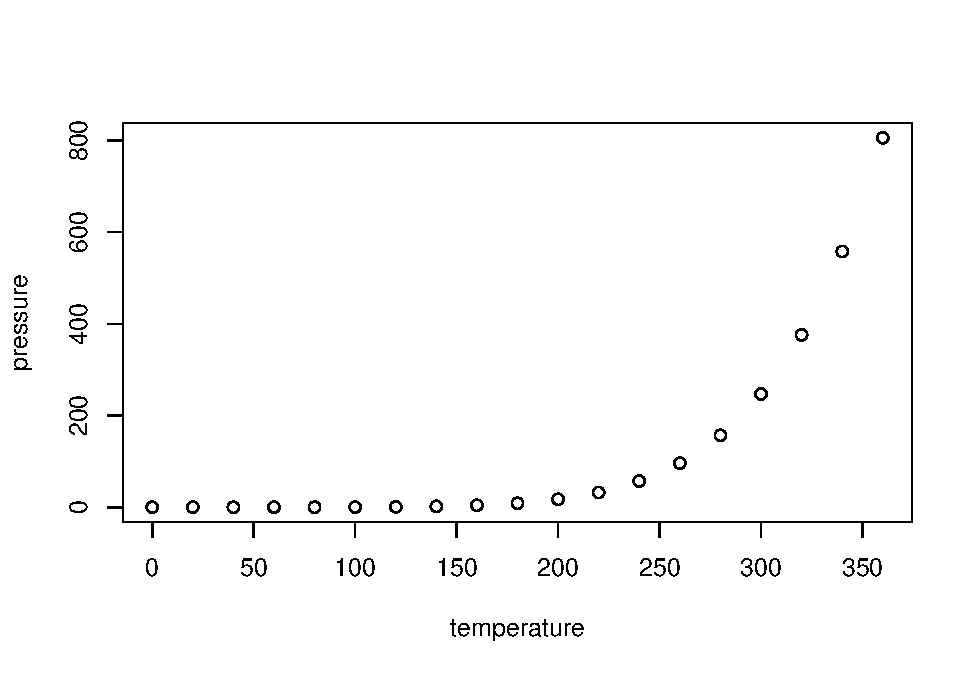
\includegraphics{Untitled_files/figure-latex/pressure-plot-1.pdf}}}
\caption{Example of a two-part figure with individual sub-captions
 showing that captions are flush left and justified if greater
 than one line of text.} \label{sample-figure}
\end{figure}

To ensure that figures are correctly numbered automatically, the
\texttt{\textbackslash{}label} command should be included just after the
\texttt{\textbackslash{}caption} command, or in its argument.

The \texttt{\textbackslash{}subfigure} command requires
\texttt{subfigure.sty}, which is called in the preamble of the
\texttt{interacttfssample.tex} file (to allow your choice of an
alternative package if preferred) and included in the \textsf{Interact}
\LaTeX~bundle for convenience. Please supply any additional figure
macros used with your article in the preamble of your .tex file.

The source files of any figures will be required when the final, revised
version of a manuscript is submitted. Authors should ensure that these
are suitable (in terms of lettering size, etc.) for the reductions they
envisage.

The \texttt{epstopdf} package can be used to incorporate encapsulated
PostScript (.eps) illustrations when using PDF\LaTeX, etc. Please
provide the original .eps source files rather than the generated PDF
images of those illustrations for production purposes.

\hypertarget{tables}{%
\subsection{Tables}\label{tables}}

The \texttt{interact} class file will deal with positioning your tables
in the same way as standard \LaTeX. It should not normally be necessary
to use the optional \texttt{{[}htb{]}} location specifiers of the
\texttt{table} environment in your manuscript; you may, however, find
the \texttt{{[}p{]}} placement option or the \texttt{endfloat} package
useful if a journal insists on the need to separate tables from the
text.

The \texttt{tabular} environment can be used as shown to create tables
with single horizontal rules at the head, foot and elsewhere as
appropriate. The captions appear above the tables in the
\textsf{Interact} style, therefore the \texttt{\textbackslash{}tbl}
command should be used before the body of the table. For example,
Table\textasciitilde{}\ref{sample-table} is produced using the following
commands:

\begin{table}
\tbl{Example of a table showing that its caption is as wide as
 the table itself and justified.}
{\begin{tabular}{lcccccc} \toprule
 & \multicolumn{2}{l}{Type} \\ \cmidrule{2-7}
 Class & One & Two & Three & Four & Five & Six \\ \midrule
 Alpha\textsuperscript{a} & A1 & A2 & A3 & A4 & A5 & A6 \\
 Beta & B2 & B2 & B3 & B4 & B5 & B6 \\
 Gamma & C2 & C2 & C3 & C4 & C5 & C6 \\ \bottomrule
\end{tabular}}
\tabnote{\textsuperscript{a}This footnote shows how to include
 footnotes to a table if required.}
\label{sample-table}
\end{table}

\begin{verbatim}
\begin{table}
\tbl{Example of a table showing that its caption is as wide as
 the table itself and justified.}
{\begin{tabular}{lcccccc} \toprule
 & \multicolumn{2}{l}{Type} \\ \cmidrule{2-7}
 Class & One & Two & Three & Four & Five & Six \\ \midrule
 Alpha\textsuperscript{a} & A1 & A2 & A3 & A4 & A5 & A6 \\
 Beta & B2 & B2 & B3 & B4 & B5 & B6 \\
 Gamma & C2 & C2 & C3 & C4 & C5 & C6 \\ \bottomrule
\end{tabular}}
\tabnote{\textsuperscript{a}This footnote shows how to include
 footnotes to a table if required.}
\label{sample-table}
\end{table}
\end{verbatim}

To ensure that tables are correctly numbered automatically, the
\texttt{\textbackslash{}label} command should be included just before
\texttt{\textbackslash{}end\{table\}}.

The \texttt{\textbackslash{}toprule}, \texttt{\textbackslash{}midrule},
\texttt{\textbackslash{}bottomrule} and
\texttt{\textbackslash{}cmidrule} commands are those used by
\texttt{booktabs.sty}, which is called by the \texttt{interact} class
file and included in the \textsf{Interact} \LaTeX~bundle for
convenience. Tables produced using the standard commands of the
\texttt{tabular} environment are also compatible with the
\texttt{interact} class file.

\hypertarget{landscape-pages}{%
\subsection{Landscape pages}\label{landscape-pages}}

If a figure or table is too wide to fit the page it will need to be
rotated, along with its caption, through 90\(^{\circ}\) anticlockwise.
Landscape figures and tables can be produced using the \texttt{rotating}
package, which is called by the \texttt{interact} class file. The
following commands (for example) can be used to produce such pages.

\begin{verbatim}
\setcounter{figure}{1}
\begin{sidewaysfigure}
\centerline{\epsfbox{figname.eps}}
\caption{Example landscape figure caption.}
\label{landfig}
\end{sidewaysfigure}
\end{verbatim}

\begin{verbatim}
\setcounter{table}{1}
\begin{sidewaystable}
 \tbl{Example landscape table caption.}
  {\begin{tabular}{@{}llllcll}
    .
    .
    .
  \end{tabular}}\label{landtab}
\end{sidewaystable}
\end{verbatim}

Before any such float environment, use the
\texttt{\textbackslash{}setcounter} command as above to fix the
numbering of the caption (the value of the counter being the number
given to the preceding figure or table). Subsequent captions will then
be automatically renumbered accordingly. The
\texttt{\textbackslash{}epsfbox} command requires \texttt{epsfig.sty},
which is called by the \texttt{interact} class file and is also included
in the \textsf{Interact} \LaTeX~bundle for convenience.

Please note that if the \texttt{endfloat} package is used, one or both
of the commands

\begin{verbatim}
\DeclareDelayedFloatFlavor{sidewaysfigure}{figure}
\DeclareDelayedFloatFlavor{sidewaystable}{table}
\end{verbatim}

will need to be included in the preamble of your .tex file, after the
\texttt{endfloat} package is loaded, in order to process any landscape
figures and/or tables correctly.

\hypertarget{theorem-like-structures}{%
\subsection{Theorem-like structures}\label{theorem-like-structures}}

A predefined \texttt{proof} environment is provided by the
\texttt{amsthm} package (which is called by the \texttt{interact} class
file), as follows:

\begin{proof}
More recent algorithms for solving the semidefinite programming relaxation are particularly efficient, because they explore the structure of the MAX-CUT problem.
\end{proof}

\noindent This was produced by simply typing:

\begin{verbatim}
\begin{proof}
More recent algorithms for solving the semidefinite programming
relaxation are particularly efficient, because they explore the
structure of the MAX-CUT problem.
\end{proof}
\end{verbatim}

Other theorem-like environments (theorem, definition, remark, etc.) need
to be defined as required, e.g.~using
\texttt{\textbackslash{}newtheorem\{theorem\}\{Theorem\}} in the
preamble of your .tex file (see the preamble of
\texttt{interactcadsample.tex} for more examples). You can define the
numbering scheme for these structures however suits your article best.
Please note that the format of the text in these environments may be
changed if necessary to match the style of individual journals by the
typesetter during preparation of the proofs.

\hypertarget{mathematics}{%
\subsection{Mathematics}\label{mathematics}}

\hypertarget{displayed-mathematics}{%
\subsubsection{Displayed mathematics}\label{displayed-mathematics}}

The \texttt{interact} class file will set displayed mathematical
formulas centred on the page without equation numbers if you use the
\texttt{displaymath} environment or the equivalent
\texttt{\textbackslash{}{[}...\textbackslash{}{]}} construction. For
example, the equation \[
 \hat{\theta}_{w_i} = \hat{\theta}(s(t,\mathcal{U}_{w_i}))
\] was typeset using the commands

\begin{verbatim}
\[
 \hat{\theta}_{w_i} = \hat{\theta}(s(t,\mathcal{U}_{w_i}))
\]
\end{verbatim}

For those of your equations that you wish to be automatically numbered
sequentially throughout the text for future reference, use the
\texttt{equation} environment, e.g. \begin{equation}
 \hat{\theta}_{w_i} = \hat{\theta}(s(t,\mathcal{U}_{w_i}))
\end{equation} was typeset using the commands

\begin{verbatim}
\begin{equation}
 \hat{\theta}_{w_i} = \hat{\theta}(s(t,\mathcal{U}_{w_i}))
\end{equation}
\end{verbatim}

Part numbers for sets of equations may be generated using the
\texttt{subequations} environment, e.g.

\begin{subequations} \label{subeqnexample}
\begin{equation}
     \varepsilon \rho w_{tt}(s,t) = N[w_{s}(s,t),w_{st}(s,t)]_{s},
     \label{subeqnparta}
\end{equation}
\begin{equation}
     w_{tt}(1,t)+N[w_{s}(1,t),w_{st}(1,t)] = 0,
     \label{subeqnpartb}
\end{equation}
\end{subequations}

which was typeset using the commands

\begin{verbatim}
\begin{subequations} \label{subeqnexample}
\begin{equation}
     \varepsilon \rho w_{tt}(s,t) = N[w_{s}(s,t),w_{st}(s,t)]_{s},
     \label{subeqnparta}
\end{equation}
\begin{equation}
     w_{tt}(1,t)+N[w_{s}(1,t),w_{st}(1,t)] = 0,   \label{subeqnpartb}
\end{equation}
\end{subequations}
\end{verbatim}

Displayed mathematics should be given end-of-line punctuation
appropriate to the running text sentence of which it forms a part, if
required.

\hypertarget{math-fonts}{%
\subsubsection{Math fonts}\label{math-fonts}}

\hypertarget{superscripts-and-subscripts}{%
\paragraph{Superscripts and
subscripts}\label{superscripts-and-subscripts}}

Superscripts and subscripts will automatically come out in the correct
size in a math environment (i.e.~enclosed within
\texttt{\textbackslash{}(...\textbackslash{})} or \texttt{\$...\$}
commands in running text, or within
\texttt{\textbackslash{}{[}...\textbackslash{}{]}} or the
\texttt{equation} environment for displayed equations). Sub/superscripts
that are physical variables should be italic, whereas those that are
labels should be roman (e.g.~\(C_p\), \(T_\mathrm{eff}\)). If the
subscripts or superscripts need to be other than italic, they must be
coded individually.

\hypertarget{upright-greek-characters-and-the-upright-partial-derivative-sign}{%
\paragraph{Upright Greek characters and the upright partial derivative
sign}\label{upright-greek-characters-and-the-upright-partial-derivative-sign}}

Upright lowercase Greek characters can be obtained by inserting the
letter \texttt{u} in the control code for the character,
e.g.~\texttt{\textbackslash{}umu} and \texttt{\textbackslash{}upi}
produce \(\umu\) (used, for example, in the symbol for the unit microns
-- \(\umu\mathrm{m}\)) and \(\upi\) (the ratio of the circumference of a
circle to its diameter). Similarly, the control code for the upright
partial derivative \(\upartial\) is \texttt{\textbackslash{}upartial}.
Bold lowercase as well as uppercase Greek characters can be obtained by
\texttt{\{\textbackslash{}bm\ \textbackslash{}gamma\}}, for example,
which gives \({\bm \gamma}\), and
\texttt{\{\textbackslash{}bm\ \textbackslash{}Gamma\}}, which gives
\({\bm \Gamma}\).

\hypertarget{acknowledgements}{%
\section*{Acknowledgement(s)}\label{acknowledgements}}
\addcontentsline{toc}{section}{Acknowledgement(s)}

An unnumbered section,
e.g.~\texttt{\textbackslash{}section*\{Acknowledgements\}}, may be used
for thanks, etc.~if required and included \emph{in the non-anonymous
version} before any Notes or References.

\hypertarget{disclosure-statement}{%
\section*{Disclosure statement}\label{disclosure-statement}}
\addcontentsline{toc}{section}{Disclosure statement}

An unnumbered section,
e.g.~\texttt{\textbackslash{}section*\{Disclosure\ statement\}}, may be
used to declare any potential conflict of interest and included \emph{in
the non-anonymous version} before any Notes or References, after any
Acknowledgements and before any Funding information.

\hypertarget{funding}{%
\section*{Funding}\label{funding}}
\addcontentsline{toc}{section}{Funding}

An unnumbered section,
e.g.~\texttt{\textbackslash{}section*\{Funding\}}, may be used for grant
details, etc.~if required and included \emph{in the non-anonymous
version} before any Notes or References.

\hypertarget{notes-on-contributors}{%
\section*{Notes on contributor(s)}\label{notes-on-contributors}}
\addcontentsline{toc}{section}{Notes on contributor(s)}

An unnumbered section,
e.g.~\texttt{\textbackslash{}section*\{Notes\ on\ contributors\}}, may
be included \emph{in the non-anonymous version} if required. A
photograph may be added if requested.

\hypertarget{nomenclaturenotation}{%
\section*{Nomenclature/Notation}\label{nomenclaturenotation}}
\addcontentsline{toc}{section}{Nomenclature/Notation}

An unnumbered section,
e.g.~\texttt{\textbackslash{}section*\{Nomenclature\}} (or
\texttt{\textbackslash{}section*\{Notation\}}), may be included if
required, before any Notes or References.

\hypertarget{notes}{%
\section*{Notes}\label{notes}}
\addcontentsline{toc}{section}{Notes}

An unnumbered \texttt{Notes} section may be included before the
References (if using the \texttt{endnotes} package, use the command
\texttt{\textbackslash{}theendnotes} where the notes are to appear,
instead of creating a \texttt{\textbackslash{}section*}).

\hypertarget{references}{%
\section{References}\label{references}}

\hypertarget{references-cited-in-the-text}{%
\subsection{References cited in the
text}\label{references-cited-in-the-text}}

\hypertarget{the-list-of-references}{%
\subsection{The list of references}\label{the-list-of-references}}

References should be listed at the end of the main text in alphabetical
order by authors' surnames, then chronologically (earliest first). If
references have the same author(s), editor(s), etc., arrange by year of
publication, with undated works at the end. A single-author entry
precedes a multi-author entry that begins with the same name. If the
reference list contains two or more items by the same author(s) in the
same year, add a, b, etc. and list them alphabetically by title.
Successive entries by two or more authors when only the first author is
the same are alphabetized by co-authors' surnames. If a reference has
more than ten named authors, list only the first seven, followed by `et
al.'. If a reference has no author or editor, order by title; if a date
of publication is impossible to find, use `n.d.' in its place.

The following list shows some sample references prepared in the Taylor
\& Francis Chicago author-date style.

\citep{Ade09, Alb05}

\bibliographystyle{tfcad}
\bibliography{interactcadsample.bib}


\input{"appendix.tex"}


\end{document}
